\documentclass{report} \usepackage[T1]{fontenc} \usepackage[italian]{babel}
\usepackage{color}
\usepackage[type={CC},modifier={by-sa},version={4.0},]{doclicense}
\usepackage{cite}

\usepackage{graphicx}
\graphicspath{ {./media/images/} }
\usepackage{float}

\usepackage{hyperref}

\title{Title} \author{Daniele Melocchi\\Agnese Montanaro\\Matteo
Savatteri}

\begin{document}
\maketitle
\setcounter{page}{2}

Copyright Daniele Melocchi, Agnese Montanaro, Matteo Savatteri -
\the\year \doclicenseThis \thispagestyle{empty}

\tableofcontents

\chapter{Introduzione}
Questo documento presenta un ciclo di lezioni svolte in modalità
di didattica a distanza (\emph{DAD}) e
indirizzate ad una classe 1\textsuperscript{a} Liceo Scientifico,
riguardanti le basi della cinematica, il moto rettilineo uniforme
e uniformemente accelerato.

Il percorso didattico è suddiviso in tre moduli, all'interno dei quali
sono affrontati i seguenti argomenti, ordinati secondo un criterio
di complessità crescente, partendo da un approccio completamente
qualitativo, per passare ad uno via via più quantitativo:
\begin{enumerate}
\item Posizioni, istanti, distanze e intervalli temporali, leggi orarie.
\item Velocità media, velocità istantanea, moto rettilineo uniforme.
\item Accelerazione media, accelerazione istantanea, moto uniformemente
      accelerato.
\end{enumerate}

Il percorso si fonda sul \emph{modello didattico delle 5E}\cite{bybee2006bscs}.
Ogni modulo si suddivide dunque in cinque fasi, nelle quali sono presentate
attività, riflessioni, suggerimenti e problematiche affrontate, per ciascuna
di queste: \emph{engage}, \emph{explore}, \emph{explain}, \emph{extend},
\emph{evaluate}.

\section{Propedeuticità}
Al fine della buona riuscita di questo percorso, è necessario che gli
studenti coinvolti abbiano affrontato e consolidato la comprensione
dei seguenti argomenti:
\begin{itemize}
\item Operazioni algebriche elementari (es. frazioni e potenze).
\item Polinomi.
\item Equazioni di primo grado.
\item Rappresentazioni di numeri su un asse ordinato.
\item Rappresentazione di coppie di numeri (punti) su un diagramma
      cartesiano.
\item Conoscenza di grandezze fondamentali.
      (es. lunghezza, tempo)
\item Conoscenza di unità di misura di grandezze fondamentali.
      (es. metro, secondo)
\end{itemize}

\chapter{Posizioni, Istanti e Intervalli}
Nel presente modulo lo studente familiarizza con i concetti
di posizione, distanza, istante (inteso come
\emph{lettura di orologio}) e intervallo di tempo.
Succesivamente, guidato dal docente, esplora le relazioni
che intercorrono tra queste nozioni nel contesto del moto di
un corpo, giungendo ad una comprensione qualitativa dei
concetti di \emph{evento} e \emph{legge oraria}.

\section{Engage}
\begin{itemize}
\item \textbf{Tempo richiesto:} 15 min.
\item \textbf{Materiale:} Computer
\end{itemize}

Il docente mostra agli studenti
\footnote{
Nel contesto della DAD, il docente può utilizzare
una piattaforma web di videotelefonia, che supporti la condivisione
di file multimediali. Jitsi Meet\textsuperscript{\textregistered},
Zoom\textsuperscript{\textregistered},
Google Meet\textsuperscript{\textregistered} e
Microsoft Teams\textsuperscript{\textregistered}
sono solo alcuni esempi.
}
il video di un fenomeno fisico riprodotto \emph{in reverse} (ovvero ribaltando
l'asse temporale). Il fenomeno fisico rappresentato dovrebbe essere scelto
in modo che sia difficile (o impossibile) distinguere se il video viene
riprodotto in reverse oppure no. Il moto di un pendolo semplice,
di un \emph{pendulum wave} o di altri moti periodici costituiscono buoni
esempi.

Nel contesto di questo progetto si è scelto il video in \emph{slow motion}
di un colibrì in volo, che si nutre da un tubicino (Figura \ref{fig:hummingbird}) 
\footnote{
\`E possibile scaricare il video presso
\href{https://github.com/savaroskij/PED1/blob/master/progetto_finale/media/video/Hummingbird.mp4?raw=true}{questa pagina web}
. L'indirizzo del video originale si trova nella bibliografia\cite{hbird}.
}
. Solamente la componente video, e non quella audio, è stata invertita per
aumentare l'effetto di inganno.

\begin{figure}
\centering
  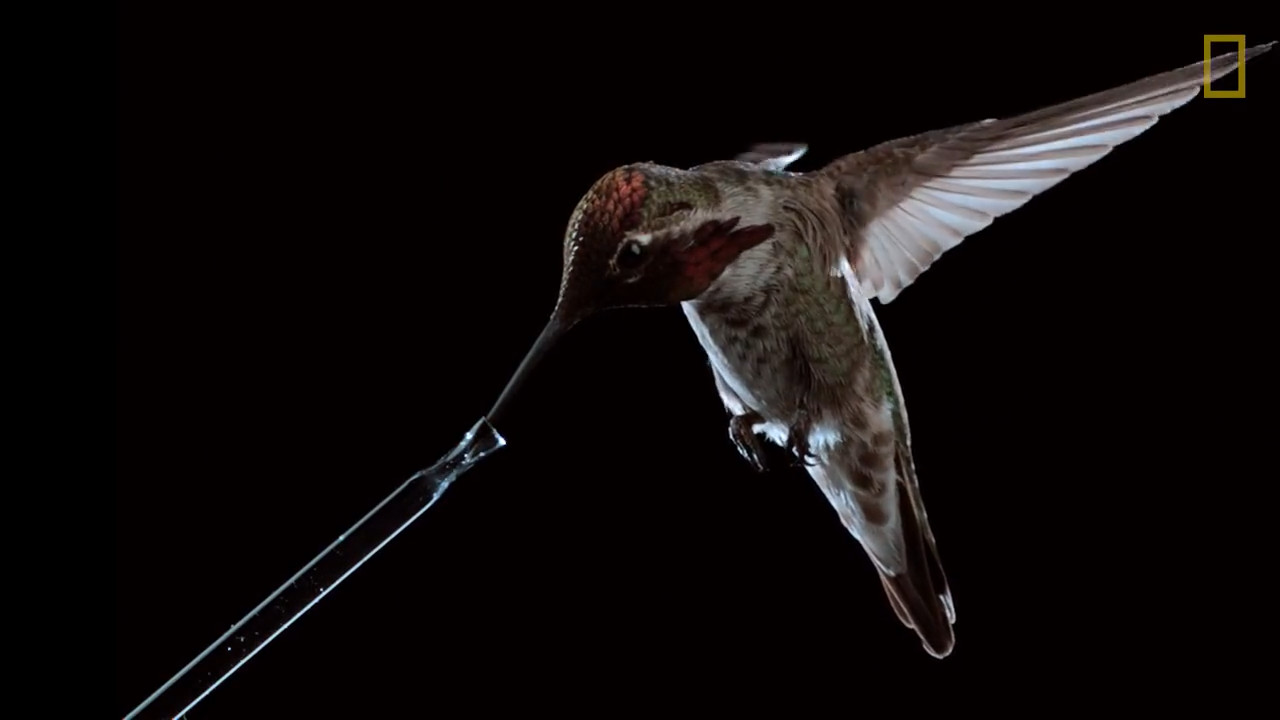
\includegraphics[width=\textwidth]{Hummingbird}
  \caption{Un frame del video di un colibrì in volo che si nutre da un tubicino.}
  \label{fig:hummingbird}
\end{figure}

Il docente in seguito chiede agli studenti di descrivere quanto viene
visualizzato, e solamente infine svela che il video è riprodotto in
reverse. In questo modo l'insegnante ha l'occasione di far notare
allo studente, e lo esplicita, che per studiare qualsiasi fenomeno fisico
occorrono chiari riferimenti spaziali e temporali.

\section{Extend}
\begin{itemize}
\item \textbf{Tempo richiesto:} 30 min.
\item \textbf{Materiale:} Computer, Oggetti domestici
\end{itemize}

In questa fase si proprone un attività mirata ad estendere la consapevolezza
degli studente riguardo ad alcuni concetti presentati precedentemente.
In particolare si desidera estendere l'idea di posizione, che lo studente ha maturato,
allo spazio tridimensiosale.

L'insegnante chiede a ciascuno studente di scegliere un oggetto nella stanza e di
spiegare alla classe, con le proprie parole, dove questo eggetto si trovi.
Lo studente potrebbe utilizzare altri oggetti nella stanza come riferimenti spaziali,
dicendo ad esempio ``L'oggetto si trova accanto alla finestra'', oppure
``L'oggetto si trova sopra il tavolo''; o forse potrebbe usare se stesso come
riferimento affermando ``L'oggetto si trova alla mia destra, in alto''.
A questo punto il docente chiede di scegliere altri due o tre oggetti,
e fa la stessa richiesta di localizzazione. Lo studente si renderà
conto dell'impossibilità di creare nella propria mente un'idea della stanza
degli altri compagni e della posizione di tutti gli oggetti, senza che
costoro esplicitino un riferimento spaziale univoco, e per ogni oggetto indichino tre distanze
misurate o stimate dal riferimento scelto.
L'insegnante dovrebbe guidare gli studenti in questo processo ponendo domande e fornendo suggerimenti
come: ``Dove si trova l'oggetto A rispetto all'oggetto B? E rispetto all'oggetto C?'',
oppure ``Dire che l'oggetto A si trova un metro sopra l'oggetto B è sufficiente
a far comprendere al tuo compagno la posizione dell'oggetto B all'interno della stanza?''
e ancora ``Forse potremmo dire che l'ogetto B si trova sopra l'oggetto A, ma anche alla sua destra
e qualche metro più avanti''.
Al termine di questo processo, il docente ufficializza la conoscenza acquisita disegnando
\footnote{
Il professore può disegnare su una lavagna e filmarsi durante l'operazione, oppure
utilizzare una tavolatta grafica o una lavagna virtuale (presente in software
come Zoom\textsuperscript{\textregistered}, ad esempio)
}          
un diagramma cartesiano tridimensionale, collocando alcuni oggetti al suo interno
e osservando che la posizione dell'oggetto preso come riferimento per tutti gli altri
si chiama \emph{origine} e le tre distanze sono rappresentate da tre numeri lungo
gli assi, chiamati \emph{coordinate cartesiane} tridimensionali.

\appendix
\chapter{Analisi Dati}
\section{Moto Rettilineo Uniforme}

\begin{figure}[H]
\centering
  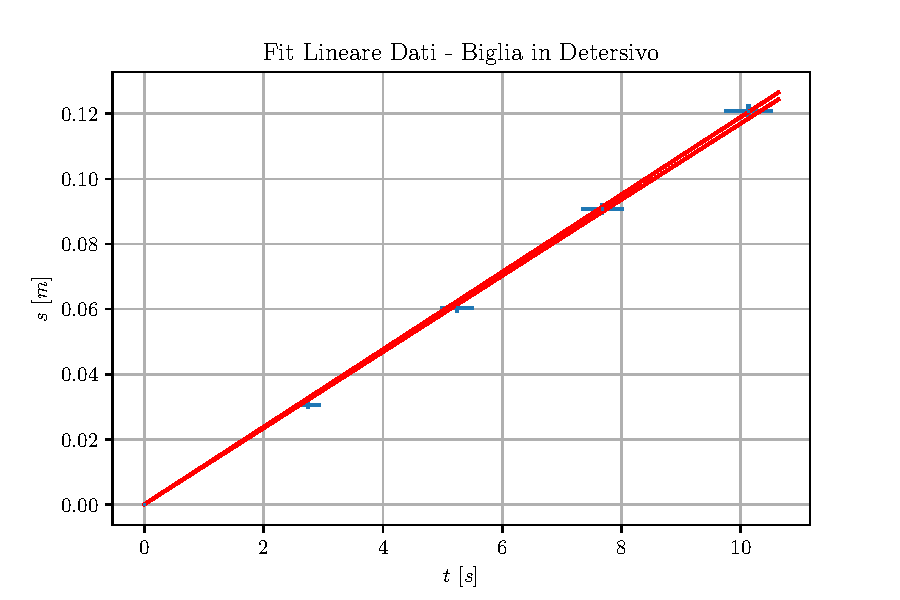
\includegraphics[width=\textwidth]{fit_marble}
  \caption{Fit lineare dei dati per l'esperimento della biglia che cade nel detersivo,
           un esempio di moto rettilineo uniforme.}
  \label{fig:fit_marble}
\end{figure}

\begin{table}[H]
  \renewcommand{\arraystretch}{1.5}
  \centering
  \begin{tabular}{ | c | }
    \hline
    $v$ [$m/s$] \\
    \hline
    $0.01180\pm0.00010$ \\
    \hline
  \end{tabular}
  \caption{Valore atteso ed errore della velocità da fit con il metodo dei minimi
           quadrati.}
  \label{tab:fit_marble}
\end{table}

\section{Moto Rettilineo Uniformemente Accelerato}

\begin{figure}[H]
  \centering
  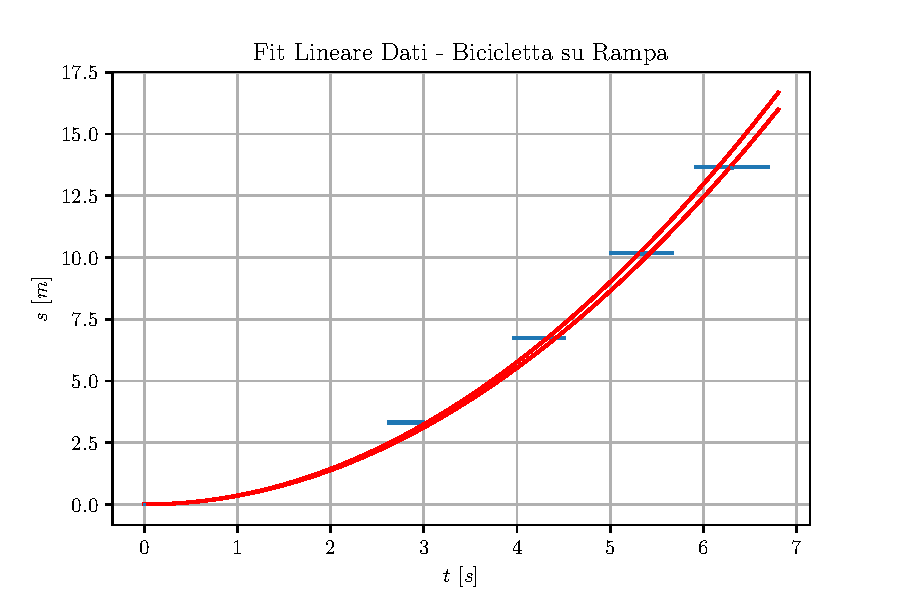
\includegraphics[width=\textwidth]{fit_bike}
  \caption{Fit lineare dei dati per l'esperimento della bicicletta che scende da una rampa,
           un esempio di moto rettilineo uniformemente accelerato.}
  \label{fig:fit_bike}
\end{figure}

\begin{table}[H]
  \renewcommand{\arraystretch}{1.5}
  \centering
  \begin{tabular}{ | c | c | c | }
    \hline
    $a$ [$m/s^2$] &  $\theta$ [deg] & pendendenza [\%] \\
    \hline
    $0.706\pm0.015$ & $4.13\pm0.09$ & $7.21\pm0.15$ \\
    \hline
  \end{tabular}
  \caption{Valore atteso ed errore dell'accelerazione, dell'angolo di inclinazione della rampa
           e della pendenza percentuale da fit con il metodo dei minimi quadrati.}
  \label{tab:fit_bike}
\end{table}

\bibliography{bibliografia}{}
\bibliographystyle{plain}
\addcontentsline{toc}{chapter}{Bibliografia}

\end{document}
